\chapter{Configuration Optimization}\label{ch:configuration_optimization}
We have now defined both a UPPAAL model, which allows us to rate configurations through simulation, as well as a set of formal transformation rules that allow us to generate new configurations. When given a set of modules and an order, these tools allow us to search through an expanding set of candidate configurations, which we can compare through their ratings. This chapter will explain how we implement this search using python.

\section{UPPAAL model Generation}
As seen in \cref{app:festoex}, to set up a single configuration in UPPAAL requires a lot of work. UPPAAL saves a system definition along with templates to an XML file. We are able to set up new configurations within UPPAAL by altering this file. Being able to generate this XML file for any configuration that we want to simulate and rate is needed in order to implement our search.

This generation is implemented with the \textit{generate\_xml} function, which can be found in the generate\_xml.py file along with all its helping functions. We will not go in depth with how it works, however its prototype can be seen in \cref{code:xmlgenerator}. As arguments it takes the path to the XML file \textit{template\_file}, a list of \textit{SquareModule} objects \textit{modules}, list of \textit{Recipe} objects \textit{recipes}. In addition, it needs the path, where to write the new XML file \textit{xml\_name} and the path, where to write the file containing the query to be run on the configuration \textit{q\_name}. This is the query run on the configuration to check if all items in the given order can be completed. 

\lstinputlisting[language=Python, caption= Prototype of the \textit{generate\_xml function}, captionpos = b, label={code:xmlgenerator}]{codeRelated/Python/xml_generator.py}

\textit{Recipe} and \textit{SquareModule} are python classes, which we have defined in order to help us set up orders and configurations. 

The prototype of \textit{Recipe}'s constructor can be seen in \cref{code:recipe}. To insantiate, we need the recipe's name \textit{name}, a dictionary describing the recipe's acyclical dependency graph \textit{dependencies}, name of module to start on \textit{start\_module}, direction to enter the start module from \textit{start\_direction} and the amount of items needed to be produced according to this recipe. Thus a list of \textit{Recipe} objects actually describes an order.

\lstinputlisting[language=Python, caption= Prototype of the \textit{Recipe} class, captionpos = b, label={code:recipe}]{codeRelated/Python/recipe.py}

The prototype of \textit{Module}'s constructor can be seen in \cref{code:module}. To instantiate, we need the module's name \textit{m\_id}, a dictionary mapping names of work to the amount of time it takes to perform and a 4 by 4 array describing transport time \textit{t\_time}. In addition, we must set the length of the module's queue in \textit{queue\_length}, as well as setting the boolean \textit{pass\_through} to indicate, wheter we can pass through this module, while it is working. To each of the parameters \textit{up}, \textit{down}, \textit{left}, \textit{right} we can assign at most one neighbour module, which this module may pass items to. To make a configuration, we connect different modules through these last four parameters.

 \lstinputlisting[language=Python, caption= Prototype of the \textit{SquareModule} class, captionpos = b, label={code:module}]{codeRelated/Python/module.py}

When we have a list of \textit{Recipe} objects, describing an order, and a list of connected \textit{Module} objects, describing a configuration, we may get the configuration rating by calling the \textit{get\_best\_time} function found in \textit{uppaalAPI.py}. This can be seen in \cref{code:get_best_time}. The function first generates a new XML file and query file from the configuration and its order using \textit{generate\_xml}. During this generation, the names of modules, works and items are translated to numerical ids in UPPAAL. The \textit{generate\_xml function} returns three dictionaries, which are mappings from the new module, work and item names to the old ones.   

It then runs the UPPAAL model checker through the verifyta executable directly on the generated XML file and query file. This is done with the \textit{run\_verifyta} function. It also takes a few additional arguments to run the verifyta executable. t2 means that we want the fasest trace, o3 means that we perform an optimal first search, u means that we want a result summary, and y makes sure that we get the trace.

This returns two strings, result and trace. From result we extract the rating using the \textit{trace\_time} function. Additionally, we send the trace to the \textit{get\_traversal\_info} function along with the name mappings from before. This analyses the trace, including all states and transitions, and extrac0st useful information about production. This includes a map from modules to the items that they work on \textit{worked\_on}. The map from module names, to items they transport \textit{transported\_through}. We also get the mapping from modules to their active works set, mentioned in \cref{ch:configuration}, \textit{active\_works}. This is used to update the module objects in the configuration according to the work that they have actually done on items. These mappings are returned from the function along with the rating.

\begin{minipage}{\linewidth}
  \lstinputlisting[language=Python, caption= \textit{get\_best\_time} function, captionpos = b, label={code:get_best_time}]{codeRelated/Python/get_best_time.py}
\end{minipage}

With these objects and functions, we have now introduced the basic constructs used to set up configurations and orders through python, as well as how to extract the ratings from configurations. As to get an idea of how they can be applied, \cref{app:pythonfestoex} to generate the rating for the construct and order pair described in \cref{ssec:realcomparison}.
\section{Tabu Search}
We have now defined, how we may set up configurations and orders in python, as well as how to get the rating of a configuration producing a specific order. We now tackle the problem of finding the optimal configuration, given an order of items and a set of avaliable modules. Finding the optimal configuration can be a difficult problem to solve. Therefore we do not focus on creating an optimization algorithm, but rather a heuristic. Unlike optimization algorithms, heuristics do not guarentee a globally optimal solution. Instead it promises a locally optimal solution, which may be good enough in practice.

\subsection{Choosing a Metaheuristic}
A metaheuristic is a problem-independent technique used to develop heuristics for optimization problems. We choose to look into the local search family of metaheuristics. These describe heuristics, where we try to tackle the problem of optimizing some measure, by moving between candidate solutions to some problem. In our case the measure we want to optimize is the configuration rating, where we want to find the configuration with the minimal value.

The most basic form of local search is hill climbing. Here we perform a local search by starting from some initial candidate solution. We then generate the neighbouring solutions and compare them on their measure value. The neighbour with the best measure is chosen as the new frontier. Search continues by generating all neighbours to this solution as to compare measures and find an even better frontier. This continues until we have a frontier, where no neighbours have a better measure. This last frontier is then chosen as the best solution. The problem with this approach is that we are very likely to move into a local optima. 

Tabu Search is another type of local search developed by Fred W. Glover \cref{glover2006}. It focuses on using memory as a way of moving away from local optima that catches us, when hill climbing. Memory comes in two different flavors short term and long term. As we search, any solution that we pick as frontier is added to the short term memory, also known as a tabu list. Any solution reciding in short term memory can not be chosen as frontier. This allows us to pick neighbours, which we would otherwise have dismissed as frontiers. In addition we are allowed to pick an ill fit neighbour to be frontier, if no other neighbour optimizes our measure. Both of these constructs guide us around local optima.

Long term memory has a few different definitions. It may be used as an extension of short term memory. Both short and long term have a limited size. This means that they will have to forget old frontiers to make room for new ones. When short term memory forgets a solution, it may end up in long term memory and continue to have us steer clear of that particular solution. In other implementations long term memory is instead used to reset search. It may happen that we enter a bad search area with many low ranking local optima. To escape this, we may replace our current frontier with one found in long term memory, as to drive search into a new area.

Memories may also be defined in different ways. A memory may describe an entire solution or perhaps just a subset of attribute values for a solution. In short term memory, the later will in general exclude more possible frontiers. 

When performing a tabu search there needs to be a balance between diversification and intensivation. Hill Climbing is pure intensivations, where we constantly try to optimize our measure. Random search on the other hand is pure diversification, where there is no active attempt made to optimize our measure. Depending on implementation, many factors in a tabu search may control diversification and intensivation. As an example, the larger short term memory is, the more diversification. The smaller it is the more intensivation.


\subsection{Tabu Search Implementation}


\begin{minipage}{\linewidth}
\lstinputlisting[language=Python, caption= pseudocode showing a simplified version of the tabu search implementation, captionpos = b, label={code:psuedotabu}]{codeRelated/Python/psuedo_tabu.py}
\end{minipage}

\section{Neighbour Functions}
In this section we describe, how we implement the transformation rules described in \cref{sec:math_rules} as neighbour functions. These neighbour functions are used by our tabu search for generating frontier neighbours as shown in \cref{code:psuedotabu}. The code for these functions can be found in the \textit{neighbour\_functions} directory and the code for solving conflicts in \textit{path\_placers.py}.


\subsection{Anti-Serialization}
For anti-serialization, we decided to implement the neighbour function in such a way that it retrieves all possible anti-serializations of a randomly chosen recipe on the main line. Meaning that whenever the transformation rules, $AS_0$, $AS_1$ and $AS_2$ could be applied on the main line for a chosen recipe, we did. We then return the resulting configurations as a set of neighbours. We also take care of shadowing and adding transport modules as brought up in \cref{ssec:restrictbranch}.

We could have implemented the neighbour function for anti-serialization in such a way that it returned all possible uses of the anti-serialize transformation rules on all recipes. We however decided against this, as it could result in too many neighbours that our tabu search would have had to evaluate in one iteration.


\subsection{Parallelization}
For parallelization, we designed the neighbour function such that we get all possible largest parallelizations. This is done because. as we assume that if we can parallelize a set of modules on a line, then the neighbours that are a configuration with a subset of these modules parallelized is likely to be worse. This might not always be the case, but it is an assumption we make, so that again our tabu search will not have to perform too many evaluation in a single iteration. 

WAdditionaly, we only implemented the $Para_0$ rule, and not $Para_1$ and $Para_2$. $Para_1$ was not implemented due to how, as we hcandled items start location. As in our implementation a only give one start module to \textit{Recipe} objects. An item can only start on a single specefic module, and $Para_1$ requires that an item can start onhas the option to start in one of multiple location. $Para_2$ was not implemented due to time constraints and for the gullible notion of symmetry.


\subsection{Swap}
For swap, we implemented the neighbour function, such that we get all possible swaps. This can possible lead to a lot of neighbours having to be evaluated, if a configuration has a lot of free modules that are capable of being swapped. We can combat this, by not making the swap transformations as likely as the other transformations in our tabu search.


\subsection{Conflicts}
For our conflict solving transformation rules described in \cref{ssec:conflicts}, we implemented special functions that are capable of solving line conflicts, which a neighbour might have after being generated by either \textit{Anti-Serialization} or \textit{Parallelization}. A \textit{push\_around} function implements the $Push Around$ rule for fixing conflicts that occur due to anti-serialization. A \textit{push\_beneathe} function implements the  $Push Beneath$ rule for conflicts that occur due to parallelization. We always check the neighbours returned by our neighbour functions for conflicts and resolve them before we evaluate them. We are not interested in evalutating and comparing neighbours, which we can not physcially set up.
 

\section{Conflicts}\label{ssec:conflicts}
As mentioned back in \cref{ch:uppaalmodel}, we did not enforce the physical rules of modules to their fullest in the UPPAAL model. These entail that a module may not connect to another module, if this module is not a neighbour and if the connection would force two modules to take up the same space. The anti-serialization transformations rules can currently create configurations, where lacking module connections mean that not all recipes can be fulfilled. This problem will be solved in \cref{ssec:restrictbranch}. Furthermore both our anti-serialization and parallelization rules can cause intersections to occur as a result of adding new lines. We will solve this problem in \cref{ssec:paround} and \cref{ssec:pbeneath}.


\subsection{Restricting Branches Anti-Serialization}\label{ssec:restrictbranch}
For the anti-serialization transformation rules described in \cref{sec:as}, we did not ensure that the first and last elements of the new line can be vertically connected to the $s$ and $e$ modules on the main line. Furthermore, until now, we have imagined that no other branch has been made from our line before performing a transformation. Yet, this will not always be the case, and as such can cause some conflicts.

\subsubsection{Neighbour Errors}
Imagine a situation similar to what the rule $AS_0$ in \cref{fig:as0} describes. Here we have specific $s$ and $e$ modules chosen on the line $\Gamma_0$, and we have chosen to branch out a specific recipe $r$. Between the two modules we have $M_{s,e}$. From this we can calculate $A_{r,s,e}$ and $B_{r,s,e}$ as described before. If $0 < |B_{r,s,e}|$, then we may branch out some modules only used to work on $r$. However in  most cases $B_{r,s,e}$ will not have a size such that it can be connected directly to the $s$ and $e$ modules. We therefore modify our $AS_0$ transformation rule, as to solve this.

If $|A_{r,s,e}| + 2 > |B_{r,s,e}|$ , then the result of our $AS_0$ transformation rule will be the top of \cref{fig:astrans}. In this case, we append the new line with transport modules to make the two lines fit each other. Notice that the modules beneath the new line are marked as shadowed, i.e. coloured red. This is used in order to handle transformation conflicts as described below in \cref{sssec:shadow}. We also introduce blue rounded boxes with indexes to the top right of them. These boxes mean that anything inside of them are serialized $i$ times, where $i$ is the index given with the box. 


If $|A_{r,s,e}| + 2 \leq |B_{r,s,e}|$,  then the result of our $AS_0$ transformation rule will be the bottom of \cref{fig:astrans}, In this case we append \Gamma_0 with transporters instead of the new line as to make them fit together.

\begin{figure}[H]
	\centering
	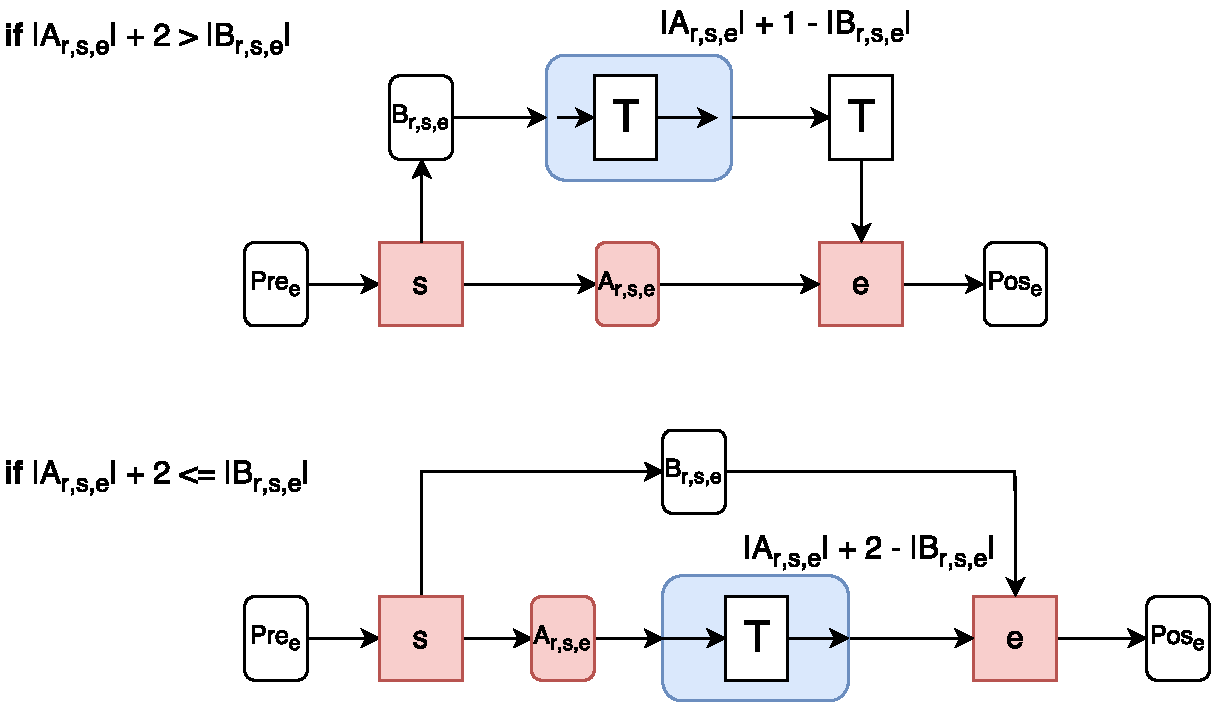
\includegraphics[width=\textwidth]{astrans.pdf}
	\caption{The new results of $AS_0$}
	\label{fig:astrans}
\end{figure}

\subsubsection{Shadowed Modules}\label{sssec:shadow}
On the top part of \cref{fig:shadowexample},  we have already made a branch from $s1$ to $e1$, which results in the modules on \Gamma_0 being shadowed. Being shadowed means that if we remove the module and just reconnect the old line as usual, then the branch becomes too long to connect back to its old line. Shadowed boxes are visualized with the colour red. The line needs to connect back to its designated point on the old line as the module located here is a common module. This module  performs work on the recipe $r$ otherwise worked on by the new line and should therefore not be bypassed. To get around this we, as shown in \cref{fig:shadowexample}, alter our anti-serialization transformation in this case to replace a shadowed module with a transport module, as not to skew the two previous lines away from each other. The example shows this done for a single module, but it may be done regardless of the amount of shadowed modules, which we remove. In \cref{fig:shadowexample} we also introduce rounded boxes with three dots in them. These boxes just means that here appears any number of modules in a total order.

As an exception, we may not remove a shadowed module, if it also used as a branching in or branching out point for some line. This means that the module is common and is used by the branch. Removing it would keep us from producing items according that branch's specific recipe. Therefore, we never allow for these modules to be removed, even if this means that we can not perform certain anti-serializations.

\begin{figure}[H]
	\centering
	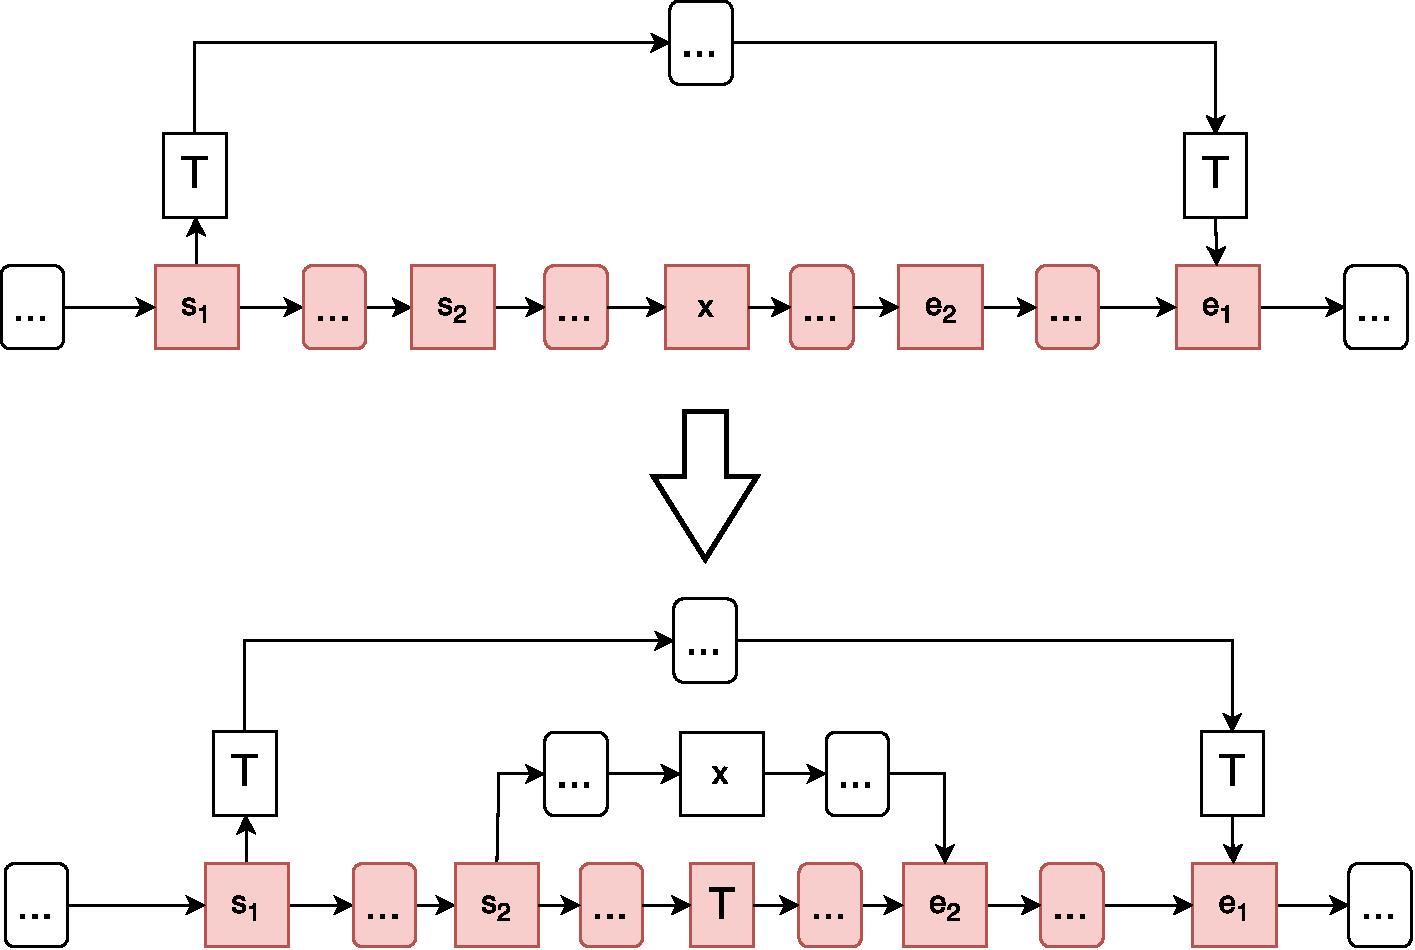
\includegraphics[width=\textwidth]{as5.pdf}
	\caption{Transformation that handles the case where an anti-serialization removes a shadowed module}
	\label{fig:shadowexample}
\end{figure}

\subsection{Push Around} \label{ssec:paround}
In push around we handle the case, where a new off branching line intersects with an old line, by moving the new line above the old line. In the case where the new line entirely covers the old, we perform the transformation depicted in \cref{fig:pusharound1}. As shown, the new line simply uses transport modules to lift itself up above the old line. These transport modules are technically not a part of the line and only serve the purpose of avoiding the intersection. If two modules are connected vertically according to either the $Start$ or $End$ functions, we may add transport modules to ensure that the described vertical path can exist.

\begin{figure}[h]
\centering
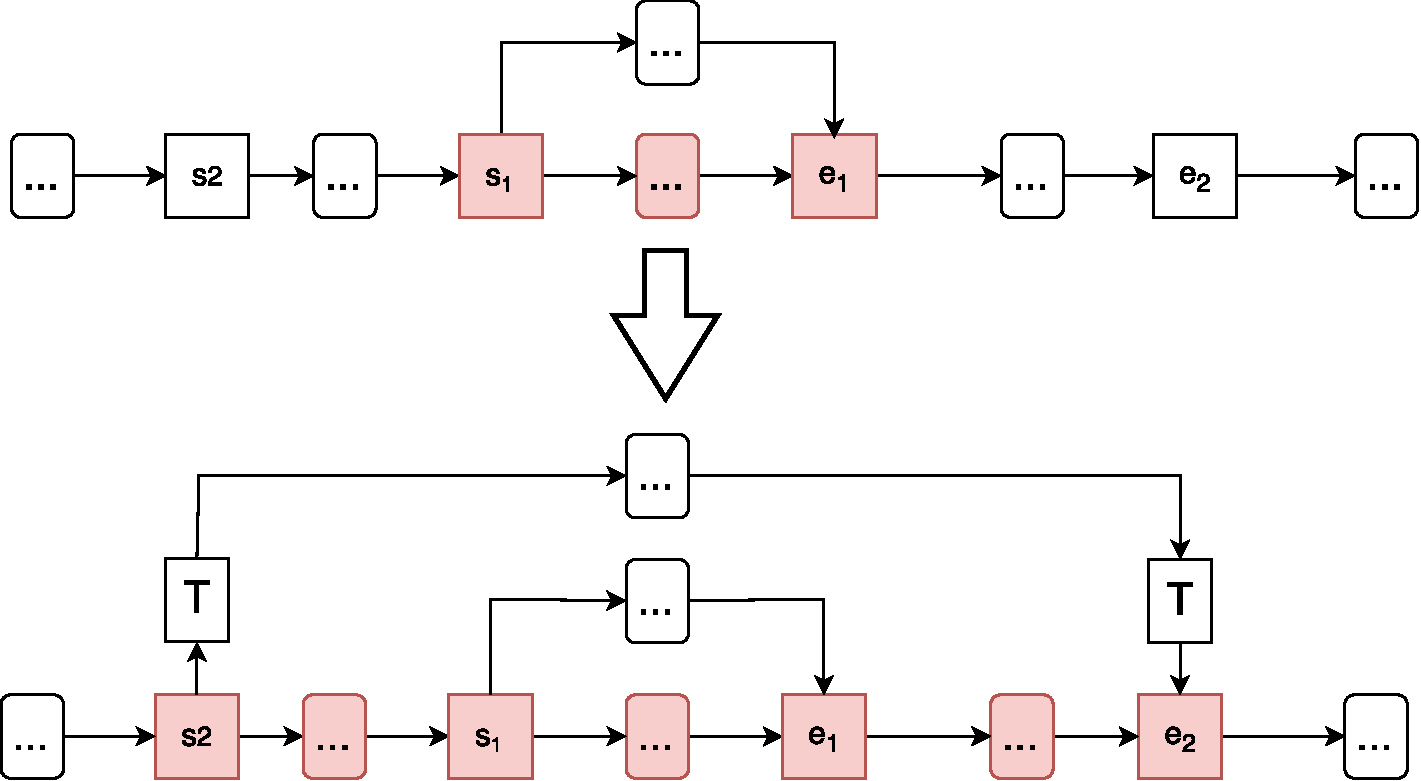
\includegraphics[width=\textwidth]{conflict1.pdf}
\caption{How Push Around handles the case, where we insert a new line that covers the entirety of an old line}
\label{fig:pusharound1}
\end{figure}

There is also the case, where the new line is covered by the old line entirely. In this case, we use the transformation in \cref{fig:pusharound2}. Here we do not need to append any transport module, as we move up through the already existing modules, which we would otherwise intersect with. 

In the cases where the new entirely intersects the old it will add transport modules where needed, or otherwise guide itself vertically through modules that already exists. These examples only show the case, where a single old line is placed above the main line, from which we branch off. In the case of more line levels, the new line will simply climb vertically until it finds a level where it may be placed without intersection. 

Push around is the intersect handling, we use when inserting new lines as a result of anti-serialization. This is chosen as there is no need to keep this new line close to \Gamma_0, from which it sprouted. 

\begin{figure}[H]
\centering
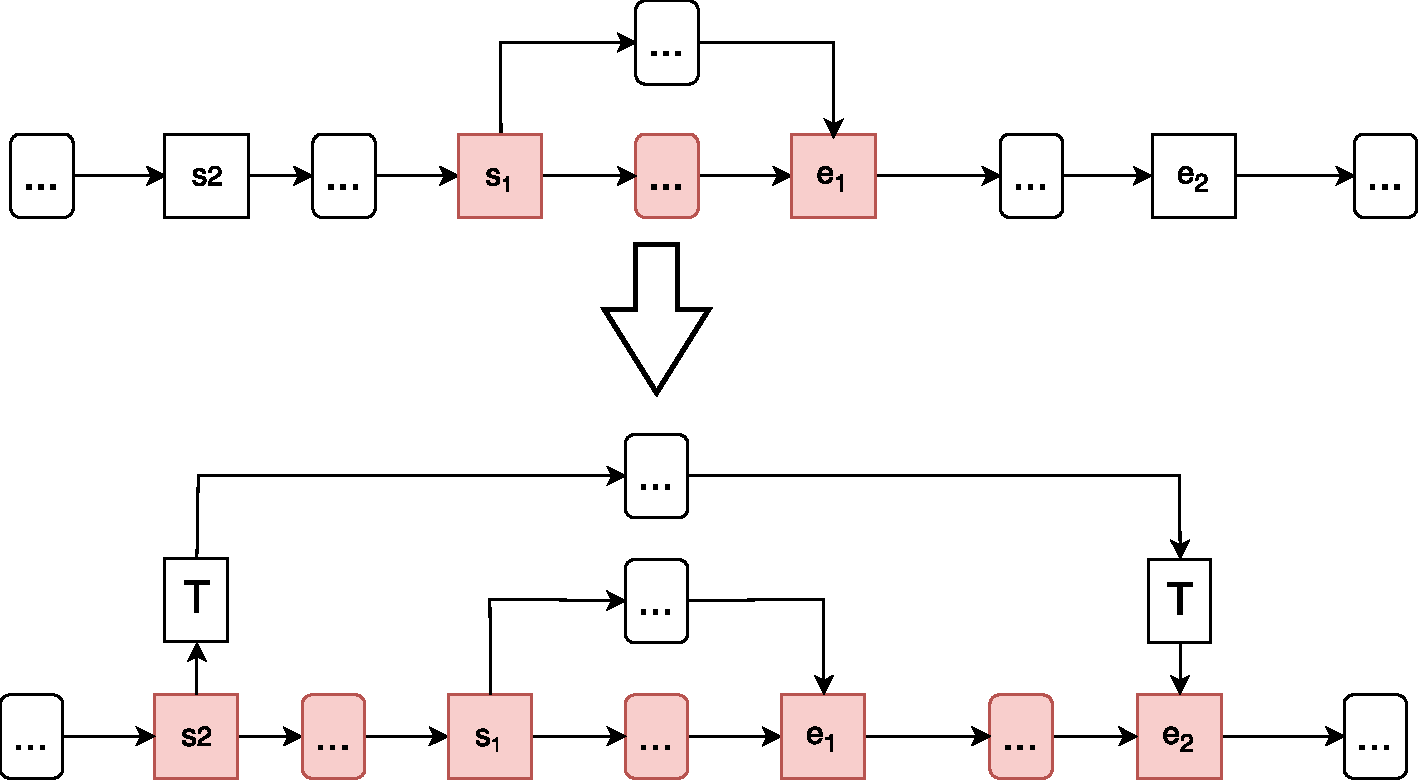
\includegraphics[width=\textwidth]{conflict2.pdf}
\caption{How Push Around handles the case, where we insert a new line that is covered by the entirety of an old line}
\label{fig:pusharound2}
\end{figure}

\subsection{Push Beneath} \label{ssec:pbeneath}
The other type of intersect handling that we use is called Push Beneath. Here we do the opposite of Push Around and handle intersection conflicts by placing the new line, where we want to place it and then moving vertically any old lines that may intersect. If this move creates another intersection we simply move the lines which we pushed into. This is done until no intersections remain. 

In the case where the new line is covered entirely by the old line we avoid intersection as in \cref{fig:pushunderneath1}. By pushing the new line up one level, we intersect the old, which needs to move up as well. This warrants that the old line gets support from transport modules.

\begin{figure}[H]
\centering
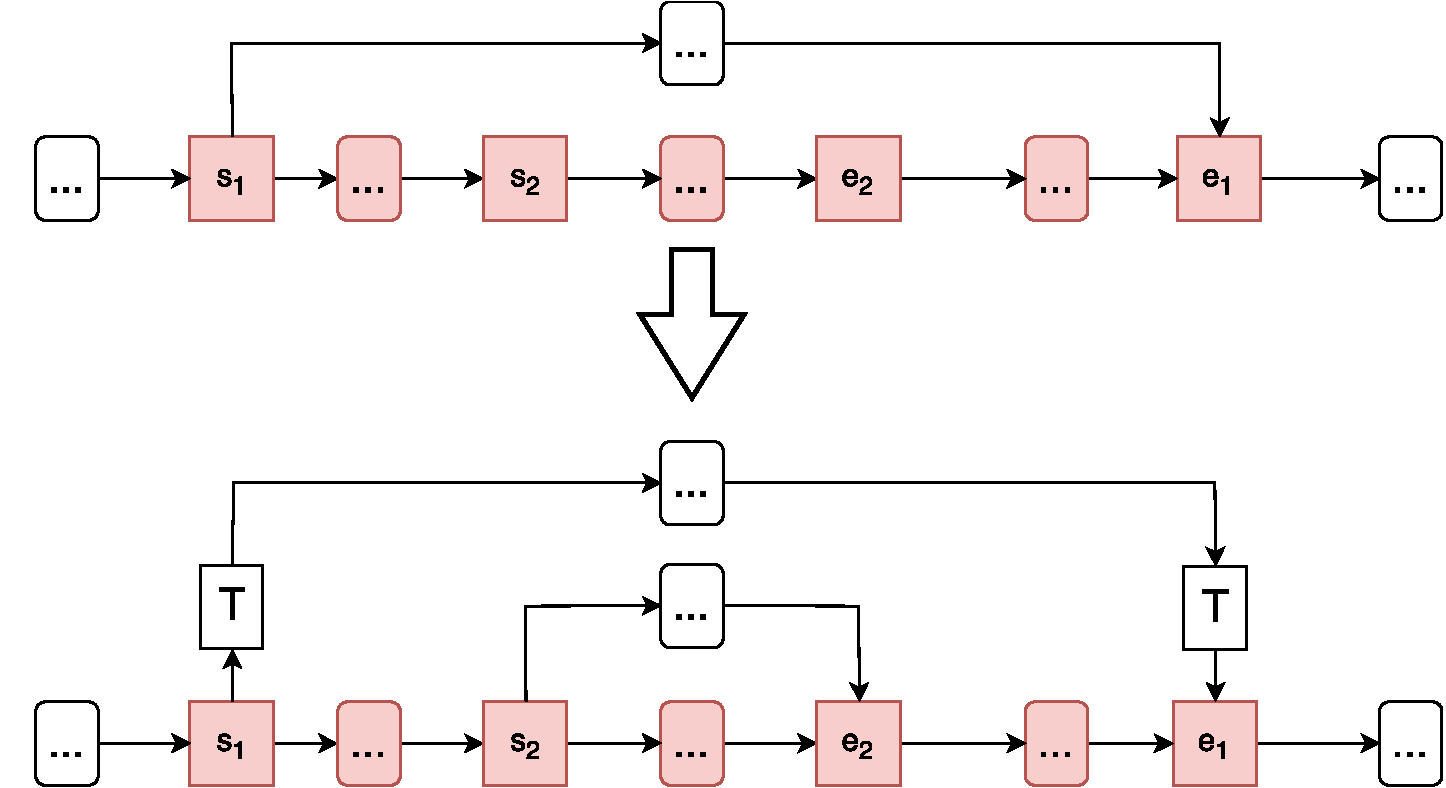
\includegraphics[width=\textwidth]{conflict3.pdf}
\caption{How Push Underneath handles the case, where we insert a new line that is covered entirely by an old line}
\label{fig:pushunderneath1}
\end{figure}

In the case, where the new line covers the old, we handle intersection as in \cref{fig:pushunderneath2}. As we push up the new line, we need to push up the old. However, we need not use transport modules to reconnect the old line, instead it can be reached by flowing vertically through the new line.

Again, the cases where there is a partial intersection between old and new line is easy to imagine. If the moving up of an old line creates a new intersection, we just move up the line that was already set in place. This is done until no more intersections occur. When this has been done, some old lines may have been disconnected from their main line. However, as these vertical connections are still included in either the $Start$ or $End$ function, transport modules may be appended, until a path has been recreated.  

As can be seen, Push Underneath functions in a manner opposite to Push Around. We decide to use it, when handling intersections that occur as a result of a parallel transformation. We want our parallel lines to be close to the line, which it sprouted from. Otherwise we may not reap the benefits of adding extra modules. This is not needed as much, when doing anti-serialization, which is why we use Push Around for that instead.

\begin{figure}[H]
\centering
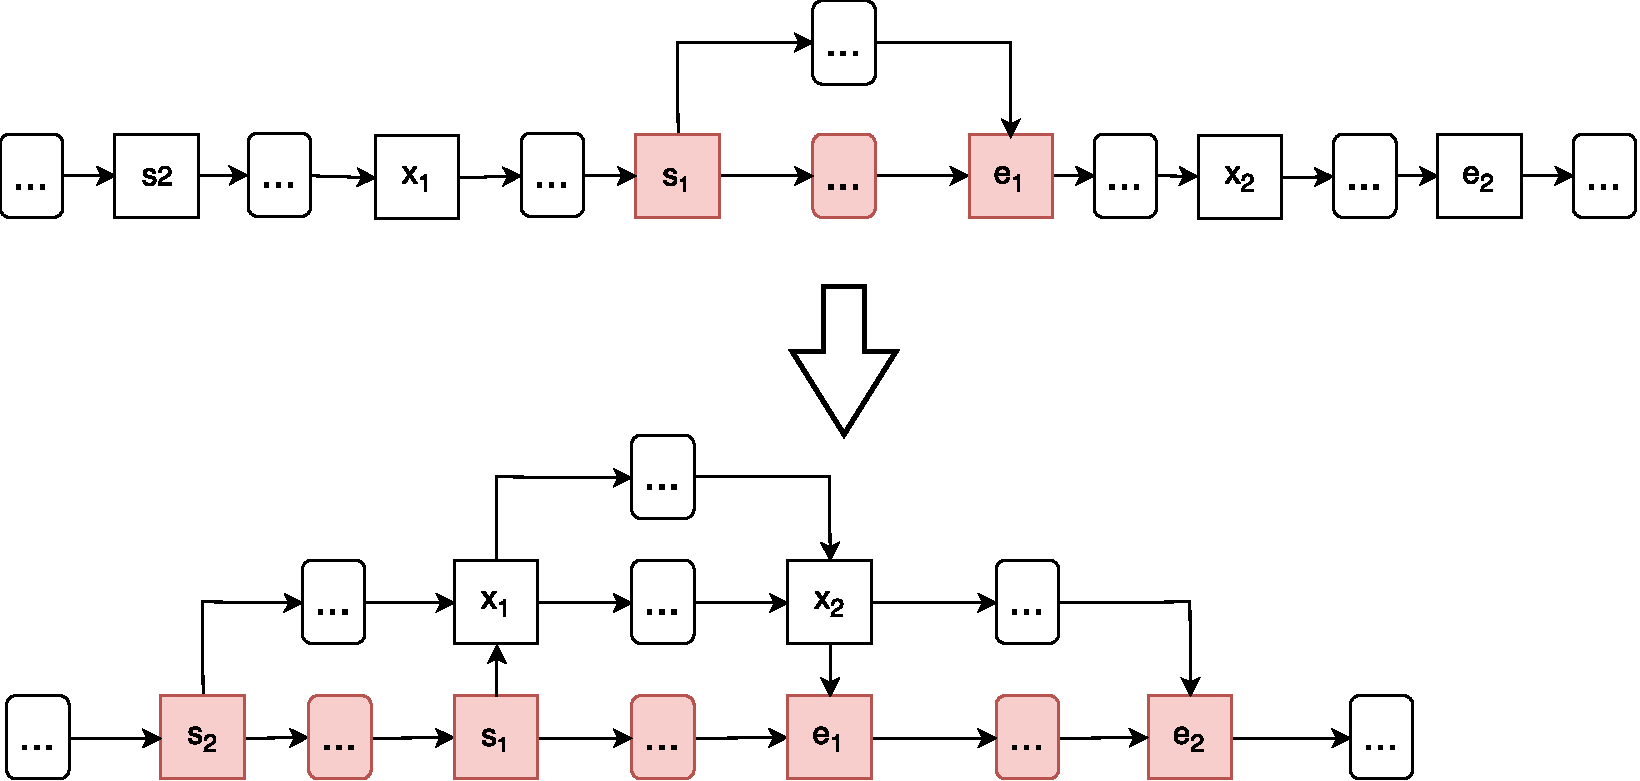
\includegraphics[width=\textwidth]{conflict4.pdf}
\caption{How Push Underneath handles the case, where we insert a new line that entirely covers an an old line}
\label{fig:pushunderneath2}
\end{figure}


\section{Generating the running example}
In this section we will use our Tabu Search on the running example first introduced in \cref{sec:runningexample}. We will present the configuration that our Tabu Search result in and compare it to the configuration that we previously made by hand.



 
